\documentclass[preprint,12pt]{aastex}
\usepackage{amsmath}

\pagestyle{empty}

\begin{document}

\section{Adiabatic winds}

In these notes, we work out the solutions for an adiabatic wind. We assume that the gas obeys $P = K \rho^\gamma$, with given constant values of the adiabatic index $\gamma$ and entropy prefactor $K$. We derive the analytic solution first and then compare with numerical results from \texttt{Athena++}.

\subsection{Sonic point}

Consider spherically-symmetric, steady, radial flow away from a star of mass $M$ and radius $R$. The continuity equation is
\begin{equation}
{1\over r^2}{d\over dr}\left(r^2\rho v\right) = 0
\end{equation}
which shows that $r^2\rho v$ is constant throughout the flow. It is convenient to write this in terms of the mass loss rate 
\begin{equation}
\dot{M} = 4\pi r^2 \rho v
\end{equation}
(which has units of $\mathrm{g\ s^{-1}}$). The momentum equation is
\begin{equation}
\rho v{dv\over dr} = -{dP\over dr}-\rho {GM\over r^2},
\end{equation}
where we assume that the gravitational acceleration is dominated by the mass of the star $M$, i.e. the self-gravity of the flow itself is negligible.

For an adiabatic flow satisfying $P=K\rho^\gamma$ with $K$ constant, we can write $dP = c^2 d\rho$ where $c^2 = \gamma P/\rho = \gamma K \rho^{\gamma-1}$ is the adiabatic sound speed. The momentum equation is therefore
\begin{equation}\label{eq:momentum}
v{dv\over dr} = -c^2{d\ln\rho\over dr}-{GM\over r^2},
\end{equation}
where we've divided through by $\rho$. Similarly, since $r^2\rho v$ is constant, we can rewrite the continuity equation as 
\begin{equation}
{d\ln\rho\over dr} = -{2\over r} -{d\ln v\over dr}.
\end{equation}
Using this to eliminate the density gradient from the momentum equation, we obtain
\begin{equation}
\left(v-{c^2\over v}\right){dv\over dr} = {2c^2\over r}-{GM\over r^2}.
\end{equation}
or
\begin{equation}
\left(1-{v^2\over c^2}\right){d\ln v\over d\ln r}=2\left({GM\over 2c^2r}-1\right).
\end{equation}
This shows that if the flow makes a transition from subsonic to supersonic, it must happen at a radius $r_s$ given by 
\begin{equation}
\boxed{
r_s = {GM\over 2c_s^2}
}
\end{equation}
where $c_s = c(r_s)$, the sound speed at $r=r_s$. This defines the location of the {\bf sonic point}.

\subsection{Energy}

Since
\begin{equation}
c^2d\ln\rho = \gamma K \rho^{\gamma-2}d\rho = {\gamma\over \gamma-1}d\left(K \rho^{\gamma-1} \right)={\gamma\over \gamma-1}d\left({P\over \rho} \right),
\end{equation}
equation (\ref{eq:momentum}) can be written
\begin{equation}\label{eq:energy}
{d\over dr}\left({1\over 2}v^2 + {\gamma \over \gamma-1}{P\over\rho} -{GM\over r}\right)=0
\end{equation}
showing that there is another constant of the flow, the energy
\begin{equation}
\boxed{
E = {1\over 2}v^2 + {c^2\over \gamma-1} -{GM\over r}
}
.
\end{equation}
Note that the middle term in equation (\ref{eq:energy}) is the enthalpy
\begin{equation}
U + {P\over \rho} = {1\over \gamma-1}{P\over\rho} + {P\over \rho} =  {\gamma \over \gamma-1}{P\over\rho},
\end{equation}
since the internal energy per unit mass of an ideal gas is given by $P = (\gamma - 1)\rho U$.

\subsection{Solution in terms of quantities at the sonic point}

By evaluating $\dot M$ and $E$ at the sonic point, we can write down a solution for the flow that depends only on the conditions at the sonic point. Starting with $\dot M$,
\begin{equation}
\dot M = 4\pi r^2 \rho v = 4\pi r_s^2 \rho_s c_s = \pi (GM)^2 {\rho_s\over c_s^3}
\end{equation}
(where a subscript s indicates that the quantity is evaluated at $r=r_s$), we find
\begin{equation}
\boxed{
\dot M =  {\pi (GM)^2\over (\gamma K)^{1/(\gamma-1)}} c_s^{5-3\gamma\over \gamma-1}.
}
\end{equation}
The energy is
\begin{equation}\label{eq:E1}
E = {1\over 2}v^2 + {c^2\over \gamma-1} -{GM\over r} = {1\over 2}c_s^2 + {c_s^2\over \gamma-1} -{GM\over r_s},
\end{equation}
which simplifies to
\begin{equation}
\boxed{
E = {c_s^2\over 2}\left({5-3\gamma\over \gamma-1}\right)
}.
\end{equation}
With the values of $\dot M$ and $E$ determined, equation (\ref{eq:E1}) can be used together with the relation
\begin{equation}
v(r) = {\dot M\over 4\pi r^2\rho(r)}
\end{equation}
to determine the profiles $v(r)$, $\rho(r)$ and $c(r)$.

\subsection{Determining the sonic point location and sound speed at the sonic point}

The previous section gives the solution for the wind in terms of the sound speed at the sonic point $c_s$, or equivalently the sonic point location $r_s$ or density $\rho_s$. We can determine the sonic point location using the conditions at the stellar surface. Evaluating $E$ at $r=R$, where the sound speed and velocity are $c_\star$ and $v_\star$ respectively, gives
\begin{equation}\label{eq:Ewithv}
E = {c_s^2\over 2}\left({5-3\gamma\over \gamma-1}\right) = {1\over 2}v_\star^2 + {c_\star^2\over \gamma-1} - {GM\over R}.
\end{equation}
For flows that start with a small Mach number, we can neglect the $v_\star$ term relative to the $c_\star$ term. Setting $v_\star =0$ gives the closed form solution
\begin{equation}
E = {c_s^2\over 2}\left({5-3\gamma\over \gamma-1}\right) = {GM\over R}\left({1\over \gamma-1}{c_\star^2 R\over GM}-1\right).
\end{equation}
Writing the Jeans escape parameter as 
\begin{equation}
\lambda_\star = {\rho_\star GM\over P_\star R} = {\gamma GM\over c_\star^2 R} = {GM\over R} {1\over K\rho_\star^{\gamma-1}},
\end{equation}
this is
\begin{equation}\label{eq:E0}
E = {c_s^2\over 2}\left({5-3\gamma\over \gamma-1}\right) = {GM\over R}\left({\lambda_\mathrm{crit}\over \lambda_\star}-1\right)
\end{equation}
where
\begin{equation}
\lambda_\mathrm{crit} = {\gamma\over\gamma-1}.
\end{equation}
The energy is positive, implying an outflow is possible, when $\lambda_\star < \lambda_\mathrm{crit}$.

The approximation that $v_\star\ll c_\star$ is good for flows that are close to isothermal $\gamma\approx 1$, but becomes less good for larger $\gamma$. In that case, we can keep the $v_\star$ term, but rewrite it in terms of $c_s$:
\begin{equation}
4\pi R^2\rho_\star v_\star = 4\pi r_s^2 \rho_s c_s\Rightarrow v_\star^2 = c_s^2 \left({r_s\over R}\right)^4\left({\rho_s\over \rho_\star}\right)^2.
\end{equation}
Defining $\tilde{E} = E/ (GM/R)$, the updated version of equation (\ref{eq:E0}) is
\begin{equation}\label{eq:tildeEeqn}
\tilde{E} = {\lambda_\mathrm{crit}\over \lambda_\star}-1 + {(2/\alpha)^\alpha\over 32}\tilde{E}^\alpha \left({\lambda_\star\over \gamma}\right)^{2/(\gamma-1)}
\end{equation}
with $\alpha = (5-3\gamma)/(\gamma-1)$. Once $\tilde{E}$ has been determined, then $c_s$ follows from
\begin{equation}\label{eq:cseqn}
c_s^2 = c_\star^2 \left({2\tilde{E}\over \alpha}\right)\left({\lambda_\star\over\gamma}\right).
\end{equation}
This shows that even when we include the $v_\star$ term, the conditions at the sonic point are determined by the single parameter $\lambda_\star$. 

As an example, it is interesting to look at the case $\gamma=7/5=1.4$ because then $\alpha=2$ and we get a quadratic equation
\begin{equation}
0 = {3125\lambda_\star^5\over 537824}\tilde{E}^2 -\tilde{E} + {7\over 2\lambda_\star}-1
\end{equation}
where we have inserted the value $\lambda_\mathrm{crit}=7/2$. As $\lambda_\star\rightarrow 7/2$, the solution has a small value of $\tilde{E}$ and the quadratic term can be neglected, we fall back to the previous solution where we assumed $v_\star=0$. This corresponds to a situation where the sonic point lies well above the stellar surface. However, as $\lambda_\star$ becomes smaller, $\tilde{E}$ increases and the quadratic term becomes important. Both roots of the quadratic converge on the value $\tilde{E}=1/2$ when $\lambda_\star = 2\gamma = 14/5$. From the definition of $\lambda_\star$, we see that this corresponds to $r_s=R$. 

More generally, 
\begin{equation}
{r_s\over R} = {GM\over 2c_s^2R} = {GM\over 2R} {\alpha\over 2E} = {\alpha\over 4\tilde{E}}
\end{equation}
(since $E = \alpha c_s^2/2$ from eq.~[\ref{eq:E0}]), so we have $r_s=R$ when $\tilde{E} = \alpha/4$. Substituting $\tilde{E}=\alpha/4$ into equation (\ref{eq:tildeEeqn}) gives
\begin{equation}
{\alpha\over 4} + 1 - {\lambda_\mathrm{crit}\over \lambda_\star} = {1\over 2^{\alpha+5}} \left({\lambda_\star\over \gamma}\right)^{2/(\gamma-1)},
\end{equation}
which is satisfied when $\lambda_\star = 2\gamma$. So we have the general behavior that $r_s/R$ starts at large values for $\lambda_\star$ just below $\lambda_\mathrm{crit}=\gamma/(\gamma-1)$, and then moves closer to the star as $\lambda_\star$ decreases. The sonic point reaches the stellar radius for $\lambda_\star=2\gamma$. 

Therefore, transonic solutions require
\begin{equation}
\boxed{
2\gamma < \lambda_\star < \lambda_\mathrm{crit} ={\gamma\over \gamma-1}.
}
\end{equation}
This range shrinks to zero at $\gamma=3/2$, so transonic solutions occur only for $1<\gamma<3/2$. It is largest for $\gamma\rightarrow 1$, in which case $\lambda_\mathrm{crit}$ diverges and there is always a wind solution no matter how small $c_\star$ becomes.

The value of the Mach number at the surface can be obtained from equation (\ref{eq:Ewithv}) and using the definition of $\lambda_\star$, which gives
\begin{equation}
\mathcal{M}_\star^2 = {2\lambda_\star\over \gamma}\left[\tilde{E} - \left(  {\lambda_\mathrm{crit}\over \lambda_\star}-1\right)\right].
\end{equation}
Note that using equation (\ref{eq:E0}) for $\tilde{E}$ gives $\mathcal{M}_\star=0$, consistent with the approximation made in deriving equation (\ref{eq:E0}). Using equation (\ref{eq:tildeEeqn}), we can rewrite this as
\begin{equation}
\mathcal{M}_\star^2 = {1\over 16}\left({2\tilde{E}\over\alpha}\right)^\alpha \left({\lambda_\star\over \gamma}\right)^{(\gamma+1)/(\gamma-1)} = {1\over 16}\left({c_s\over c_\star}\right)^{2\alpha} \left({\lambda_\star\over \gamma}\right)^4.
\end{equation}

\subsection{Hydrostatic solutions at large $\lambda_\star$}

We can get some further insight into the value of $\lambda_\mathrm{crit}$ by looking for hydrostatic solutions. With $P=K\rho^\gamma$, hydrostatic balance is  
\begin{equation}
{dP\over dr} = \gamma K \rho^{\gamma-1} {d\rho\over dr} = -\rho {GM\over r^2}.
\end{equation}
Integrating this from the stellar surface outwards,
\begin{equation}
\int_{\rho_\star}^\rho \gamma K \rho^{\gamma-2} d\rho = - \int_R^r {GM\over r^2} dr
\end{equation}
\begin{equation}
{\gamma K\over \gamma-1}\left(\rho^{\gamma-1}-\rho_\star^{\gamma-1}\right) = GM \left({1\over r} - {1\over R}\right)
\end{equation}
\begin{equation}
\left({\rho\over \rho_\star}\right)^{\gamma-1}-1 = {\lambda_\star\over \lambda_\mathrm{crit}} \left({R\over r} -1\right),
\end{equation}
or 
\begin{equation}
\left({\rho\over\rho_\star}\right)^{\gamma-1} = {\lambda_\star\over \lambda_\mathrm{crit}}\left({R\over r}-{R\over r_\mathrm{max}}\right),
\end{equation}
where the maximum extent of the atmosphere, the radius where the density drops to zero, is given by
\begin{equation}
r_\mathrm{max} = {R\over 1-\lambda_\mathrm{crit}/\lambda_\star}.
\end{equation}
Therefore we see that there is a hydrostatic solution as long as $\lambda_\star > \lambda_\mathrm{crit}$. As $\lambda_\star$ approaches $\lambda_\mathrm{crit}$ from above, the extent of the atmosphere $r_\mathrm{max}\rightarrow \infty$. For even smaller values of $\lambda_\star$, we transition into the wind solutions discussed earlier. As $\gamma\rightarrow 1$ and $\lambda_\mathrm{crit}$ diverges, we lose the hydrostatic solutions. This is consistent with the density profile of an isothermal atmosphere, which falls off exponentially. In contrast to a polytropic atmosphere, an isothermal atmosphere does not have a finite thickness. 

How do we interpret $\lambda_\star = \lambda_\mathrm{crit}$? Using the definition of $\lambda_\star$, this corresponds to
\begin{equation}
\gamma {GM\over c_\star^2 R} = {\gamma\over \gamma-1}
\end{equation}
or 
\begin{equation}
{GM\over R} = {c_\star^2\over \gamma-1},
\end{equation}
i.e. the specific enthalpy of the gas is equal to the gravitational binding energy at the surface of the star. A wind solution requires that the enthalpy be large enough to provide the gravitational energy required to take mass out to infinity, this allows $E\rightarrow v^2/2$ to be positive at infinity.

An atmosphere with $\gamma>3/2$ will develop a wind even when it still has a finite extent. For these values of $\gamma$, we have $\gamma_\mathrm{crit}<2\gamma$, so a transonic wind is not possible. Instead, once $\lambda_\star$ decreases below $2\gamma$, i.e. the sound speed at the stellar surface satisfies 
\begin{equation}
c_\star^2 > {GM\over 2R}
\end{equation}
then a supersonic wind forms. The radius of the atmosphere at this point is (substituting $\lambda_\star=2\gamma$ into the expression for $r_\mathrm{max}$)
\begin{equation}
r_\mathrm{wind} = {2(\gamma-1)R\over 2\gamma-3}.
\end{equation}
(Note that $r_\mathrm{wind}\rightarrow\infty$ for $\gamma=3/2$). 


\subsection{Numerical solutions from \texttt{Athena++}}

We ran adiabatic wind models in \texttt{Athena++}. We choose units by setting the inner edge of the numerical grid at $r=1$, ie. we measure distance in units of the stellar radius, and we choose $GM=1$ and set $\rho_\star=1$ at the surface of the star. We used 1024 logarithmically-spaced grid points from $r=1$ to $r=100$. At the inner boundary, we assume hydrostatic balance for the ghost cells, and $dv/dr=0$. At the outer boundary, we set $dv/dr=0$ and $d(r^2\rho)/dr=0$. To establish the wind, we initialize the region $R<r<1.1R$ with density $\rho_\star$, and density $10^{-14}$ on the rest of the grid, zero velocities everywhere. This results in rapid ejection of a shell and then the solution evolves to the steady-state.

Given the choice of units, we calculate analytic predictions as follows. With $\rho_\star=1$, we have $c_\star^2=\gamma K$, and $\lambda_\star = 1/K$. 
We then solve equations (\ref{eq:tildeEeqn}) and (\ref{eq:cseqn}) to find $\tilde{E}$ ($=E$ in code units) and $c_s$. The accretion rate and velocity at the surface are
\begin{equation}
\dot{M} =  {\pi\over (\gamma K)^{1/(\gamma-1)}}c_s^\alpha,\hspace{1cm}
v_\star = {c_s^\alpha \over 4} (\gamma K)^{-{3+\alpha\over 2}}.
\end{equation}

Figures 1 and 2 show the results from a set of models with $\gamma=1.4$ and $\gamma=1.1$ respectively. We find that for $K<K_\mathrm{crit}$, the numerical solution matches well with the hydrostatic profile as expected. The sonic point approaches the stellar surface as $K\rightarrow 1/2\gamma$. 


\begin{figure}
\begin{center}
	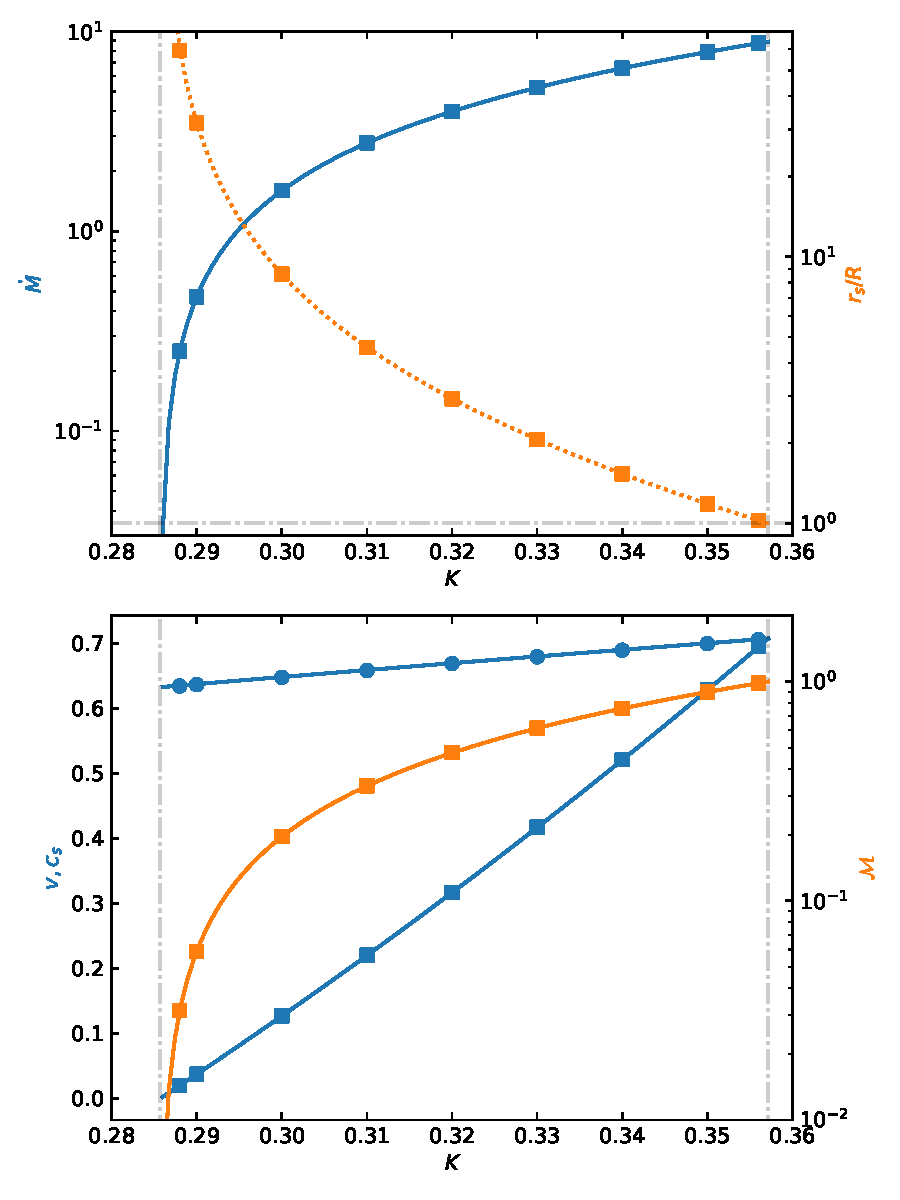
\includegraphics[width=13.5cm]{plot_gam14.pdf}
	\figcaption{Properties of the wind as a function of $K$ for transonic solutions with $\gamma=7/5$. Lines are the analytic solution for the adiabatic wind, and the symbols are the values measured from the numerical simulations. The dot-dashed lines show $r_s=R$ (horizontal line), $K = (\gamma-1)/\gamma$ (left vertical line) and $K=1/2\gamma$ (right vertical line). \label{fig:gam14}}
\end{center}
\end{figure}


\begin{figure}
\begin{center}
	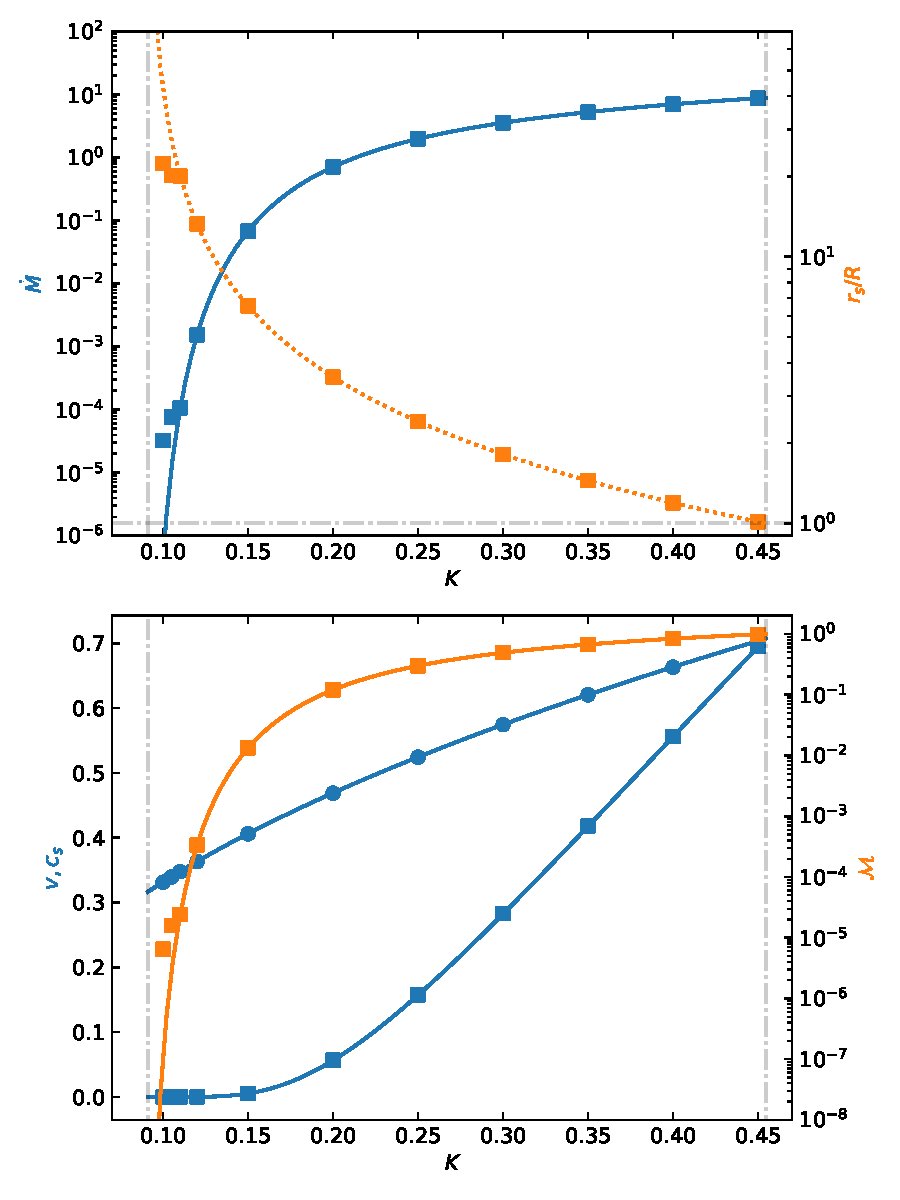
\includegraphics[width=13.5cm]{plot_gam11.pdf}
	\figcaption{Same as Figure \ref{fig:gam14} but for $\gamma=1.1$. }
\end{center}
\end{figure}



\end{document}

